\chapter{Background estimation method}\label{ch:background_method}



\section{Jet mass templates}\label{sec:jet_mass_templates}

\subsection{Template creation}\label{subsec:template_creation}

Jet mass templates are derived from a signal-depleted control region consisting of events with exactly three large-R jets.
For each $p_T$, $|\eta|$, and b-match bin, the distribution of individual jet masses in that bin is taken as the template.
The templates combine to form the binned conditional probability distribution: $p(m|p_{T}, |\eta|, b-match)$.

Separate templates are created for b-matched and non-b-matched jets.
For the b-matched templates, only events with $|\Delta \eta_{1,2}| > 1.4$ are included in the templates.
Templates derived from b-matched jets are used to dress b-matched jets in the kinematic sample,
and templates derived from non-b-matched jets are used to dress non-b-matched jets in the kinematic sample.
Each template is a one-dimensional histogram of $\log\left(m/p_{T}\right)$, with $50$ bins.
Jets with $\log\left(m/p_{T}\right)< -7$ are excluded from the templates.
Example templates are shown in figure~\ref{fig:template_examples} for two representative $p_{T}$-$|\eta|$ bins.
A clear difference can be seen between the templates derived from b-matched and non-b-matched jets.
Jets that are b-matched have a higher value of $m/p_{T}$ than non-b-matched jets, for the same  $p_{T}$-$|\eta|$ bin.
This feature can be seen in both data and simulation.
Additionally, agreement between data and simulation is observed in the general template shapes.

\begin{figure}[!ht]
    \centering
    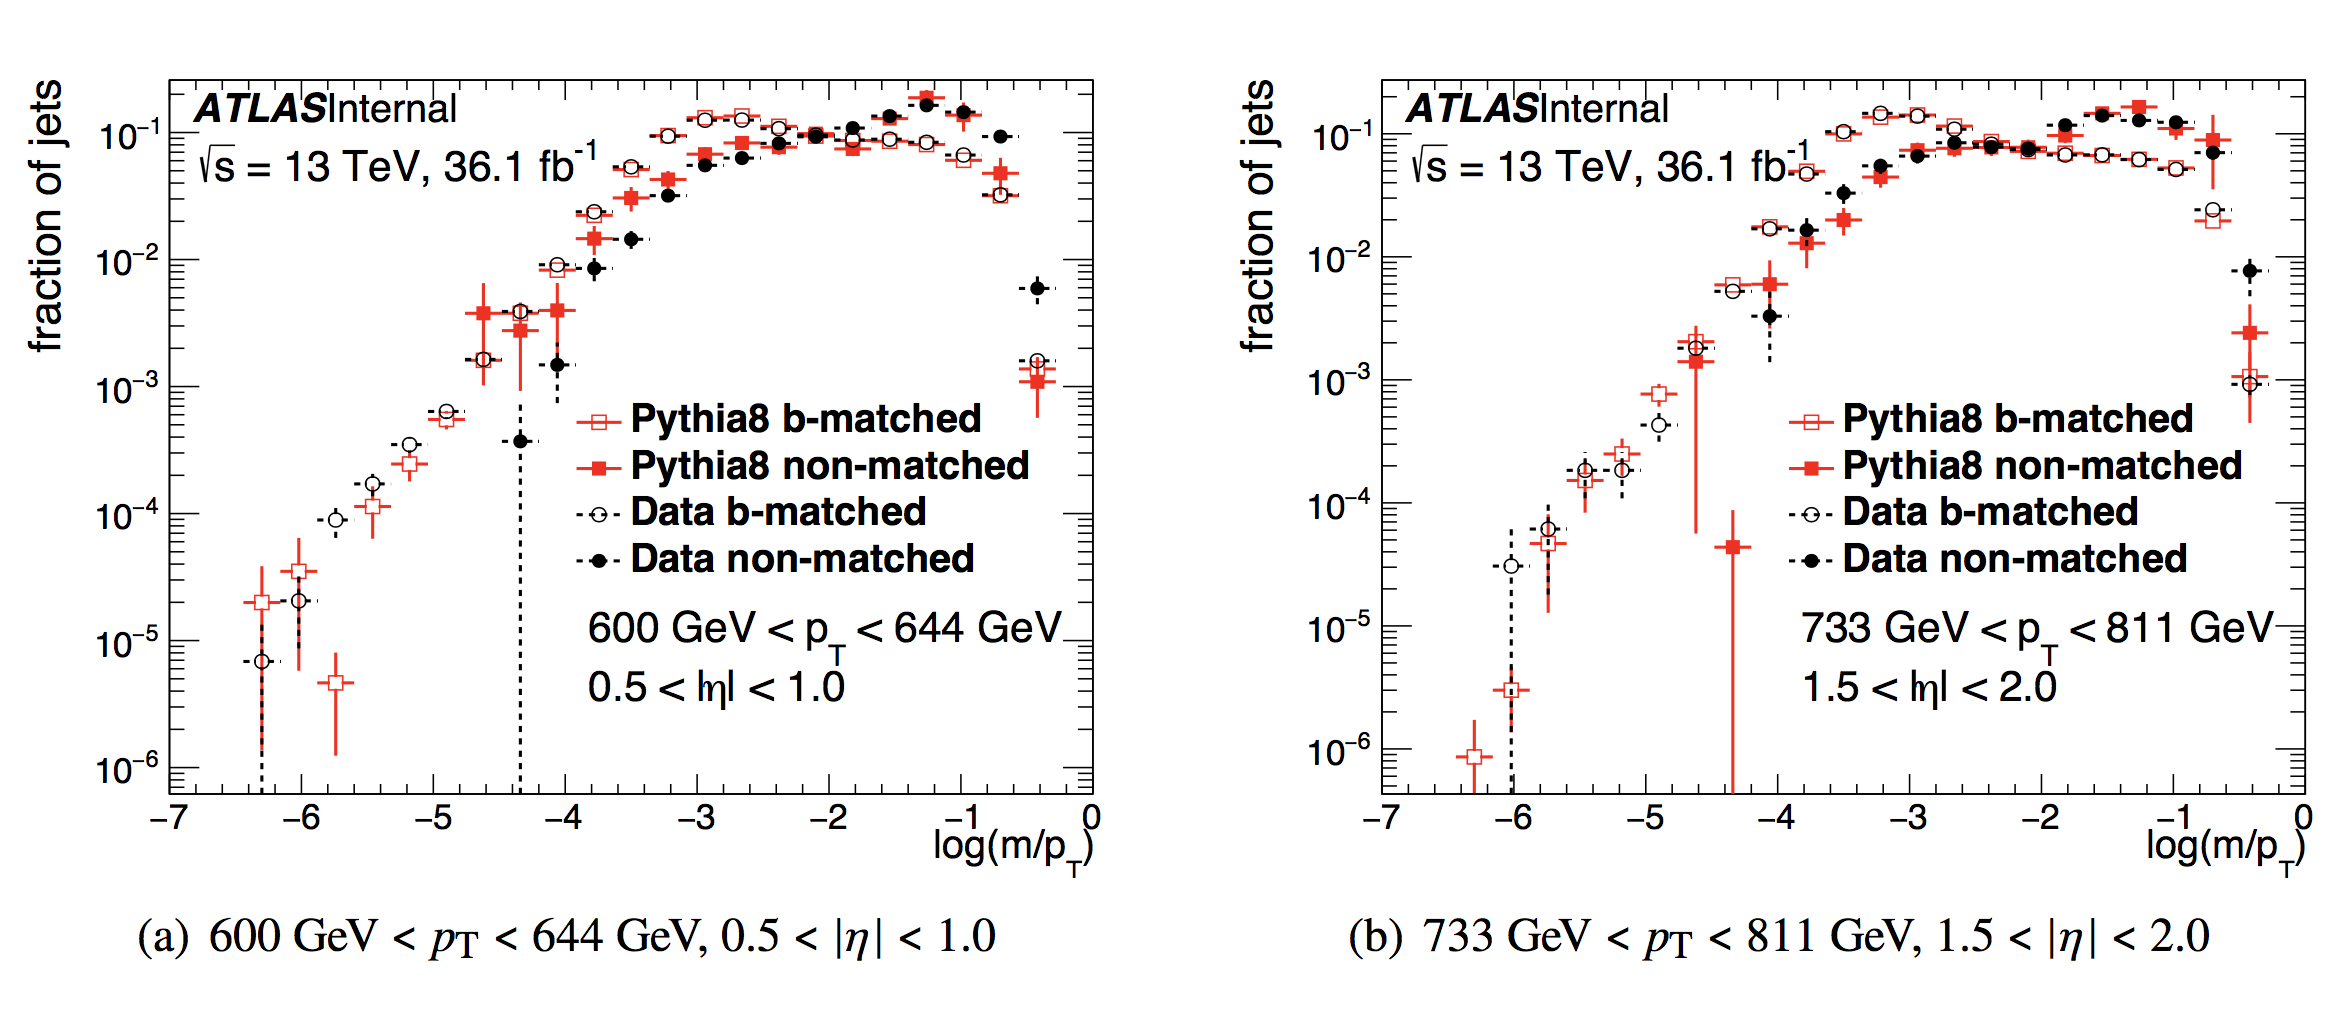
\includegraphics[width=0.9\textwidth]{template_examples}
    \caption{Two representative template distributions used in the analysis, showing a comparison between data in black and simulation in red.
    The solid markers show the templates derived from b-matched jets, while the empty markers show the templates derived from non-b-matched jets.
    In (a), template jets are required to have $600~GeV < p_{T} < 644~GeV$ and $0.5 <|\eta|<1.0$.
    In (b), templates jets are required to have $733~GeV < p_{T} < 811~GeV$ and $1.5<|\eta|<2.0$~\cite{paper-plb}.}
    \label{fig:template_examples}
\end{figure}

Templates are binned in $p_T$ and $|\eta|$.
The $p_T$ bins are approximately logarithmic, while the $|\eta|$ bin boundaries are at $0.0$, $0.5$, $1.0$, and $1.5$.
The template binning and number of jets contributing to each bin are shown in figure~\ref{fig:template_stats}.

\begin{figure}[!ht]
    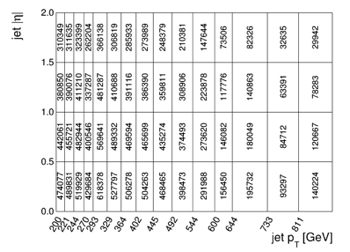
\includegraphics[width=0.45\textwidth]{template_stats_bU}
    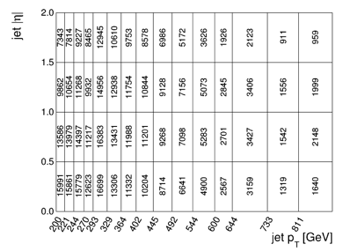
\includegraphics[width=0.45\textwidth]{template_stats_bM}
    \caption{Number of jets contributing to each template bin for the non-b-matched (left) and b-matched (right) templates.}
    \label{fig:template_stats}
\end{figure}

\subsection{Template validation} \label{subsec:template_validation}
Dressed mass response plots are created by plotting the average dressed and average kinematic jet mass in each $p_T$ bin.
The dressed mass response for the control region is shown in figure~\ref{fig:response_3jCR}.
Good agreement between average dressed and kinematic masses is observed in this region, because the dressing procedure is applied to the same jets from which the templates are derived.

Dressed mass response plots in other regions are used to evaluate how well the mass templates generalize to events with different jet multiplicities.
In the absence of signal events, a disagreement between the average dressed and kinematic masses would indicate that an individual jet mass is
dependent on the number of jets in that jet's event, violating the assumptions of the template method.
A data-driven method is used to estimate the extent to which this assumption is violated, and the size of the effect this can have on the background estimation uncertainty.
This method is described in~\ref{subsec:bkg_uncert}.

\begin{figure}[!ht]
    \centering
    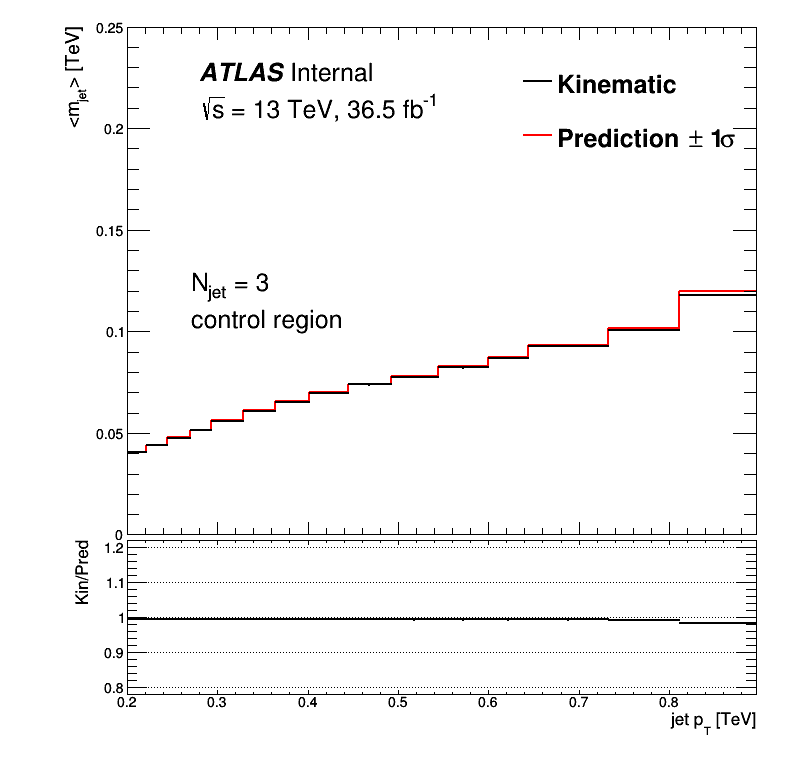
\includegraphics[width=0.6\textwidth]{plot_mass_response_3jCR}
    \centering
    \caption{Average dressed and kinematic jet masses for each $p_T$ bin
    in the control region}
    \label{fig:response_3jCR}

\end{figure}

\subsection{Background estimation using jet mass templates}\label{subsec:template_method}

For each jet in the kinematic region, a dressed mass is generated by sampling from the template corresponding to its $p_T$, $|\eta|$ and b-match bin.
To generate a dressed mass, the empirical cumulative distribution function (ECDF) is calculated for the template.
A uniform random number, $y$, in the range $[0,1)$ is then generated.
The inverse of the ECDF, $\Phi^{-1}(y)$, gives a randomized $\log\left(m/p_T\right)$ bin.
A second uniform random number, $x$, is sampled from the range $[x_1$,$x_2)$, where $x_1,x_2$ are the edges of the selected bin.
The dressed mass is then computed as $m_{dressed} = p_{T}e^x$.
To obtain a dressed $M_{J}^{\Sigma}$ for an event, one dressed mass is generated for each jet, and the dressed masses are summed.
For events with more than four jets, only the first four leading jets are included in the sum.

To obtain the nominal dressed $M_{J}^{\Sigma}$ distribution, $n_{toys}$ histograms of $M_{J}^{\Sigma}$ are created, where each histogram is generated by dressing all events in the sample once.
For each $M_{J}^{\Sigma}$ bin, the average bin content over all histograms is taken as the nominal value, and the standard deviation of bin contents is taken as one contribution to the statistical uncertainty.
The $M_{J}^{\Sigma}$ histograms are binned as follows.
There are ten equal-width bins covering the range $0~TeV \leq M_{J}^{\Sigma} < 0.5~TeV$.
The next three bins cover the ranges $0.5~TeV \leq M_{J}^{\Sigma} < 0.6~TeV$, $0.6~TeV \leq M_{J}^{\Sigma} < 0.8~TeV$, and $0.8~TeV \leq M_{J}^{\Sigma} < 1.0~TeV$.
The final bin is $M_{J}^{\Sigma} \geq 1.0~TeV$ .
The dressed $M_{J}^{\Sigma}$ distributions are scaled such that the dressed yield in the range  $0.2~TeV < M_{J}^{\Sigma} < 0.4~TeV$ is equal to the kinematic yield in the same range.
Separate scale factors are derived for each of the validation and signal regions.

To determine the nominal predicted background yield, one thousand toys are generated,
where a toy consists of a dressed $M_{J}^{\Sigma}$ value for each event in the kinematic sample.
For each toy, the number of events with dressed $M_{J}^{\Sigma}$ greater than the signal region $M_{J}^{\Sigma}$ cut are counted,
giving a distribution of one thousand dressed background yields.
The central value of this distribution is multiplied by the scale factor to obtain the nominal background prediction.
The standard deviation of this distribution is multiplied by the scale factor to obtain the statistical uncertainty on the background prediction.

Systematically-shifted background yield predictions are determined by repeating the above procedure for the systematically-shifted dressed $M_{J}^{\Sigma}$ values.
The systematic uncertainties are taken as the difference between the nominal and systematically-shifted background yield predictions.
Scale factors are only derived from the nominal $M_{J}^{\Sigma}$ distributions and applied to both the nominal and systematically-shifted predictions.
The two systematic uncertainties are symmetrized by taking the maximum of the \linebreak downward-shifted and upward-shifted uncertainties.

\subsection{Systematic uncertainty} \label{subsec:bkg_uncert}

The template method relies on the assumption that the probability density function (PDF) for a jet in a background event to have mass $m$ depends only on the jets $p_{T}$, $\eta$, and $b$-match status of the individual jet.
It also assumes that the mass PDF of a jet is independent of the masses of other jets in the event.
Because these assumptions are known to be only approximately true, the method will have some inherent bias, which should be accounted for as a systematic uncertainty.
To understand this uncertainty, signal-depleted regions called UDRs are defined, which are independent from signal and validation regions.
The predicted jet mass in these regions can be compared to the measured jet mass to determine the level of systematic uncertainty inherent to the method.

As can be seen in figure~\ref{fig:udr_response}, the dressing procedure tends to under-predict jet masses in UDR1 and over-predict jet masses in UDR2.
The degree of discrepancy depends strongly on $p_T$ and the choice of UDR .
Separate uncorrelated systematic uncertainties are derived for jets with $p_T<400~GeV$ and those with $p_T>400~GeV$.
Since the discrepancy is larger in UDR1 than UDR2 for jets with $p_T<400~GeV$, UDR1 is used to derive the uncertainty for those jets.
For jets with $p_T<400~GeV$, uncertainties are correlated across $p_T$ and $|\eta|$ bins, and likewise for jets with $p_T>400~GeV$.

\begin{figure}[!ht]
    \centering
    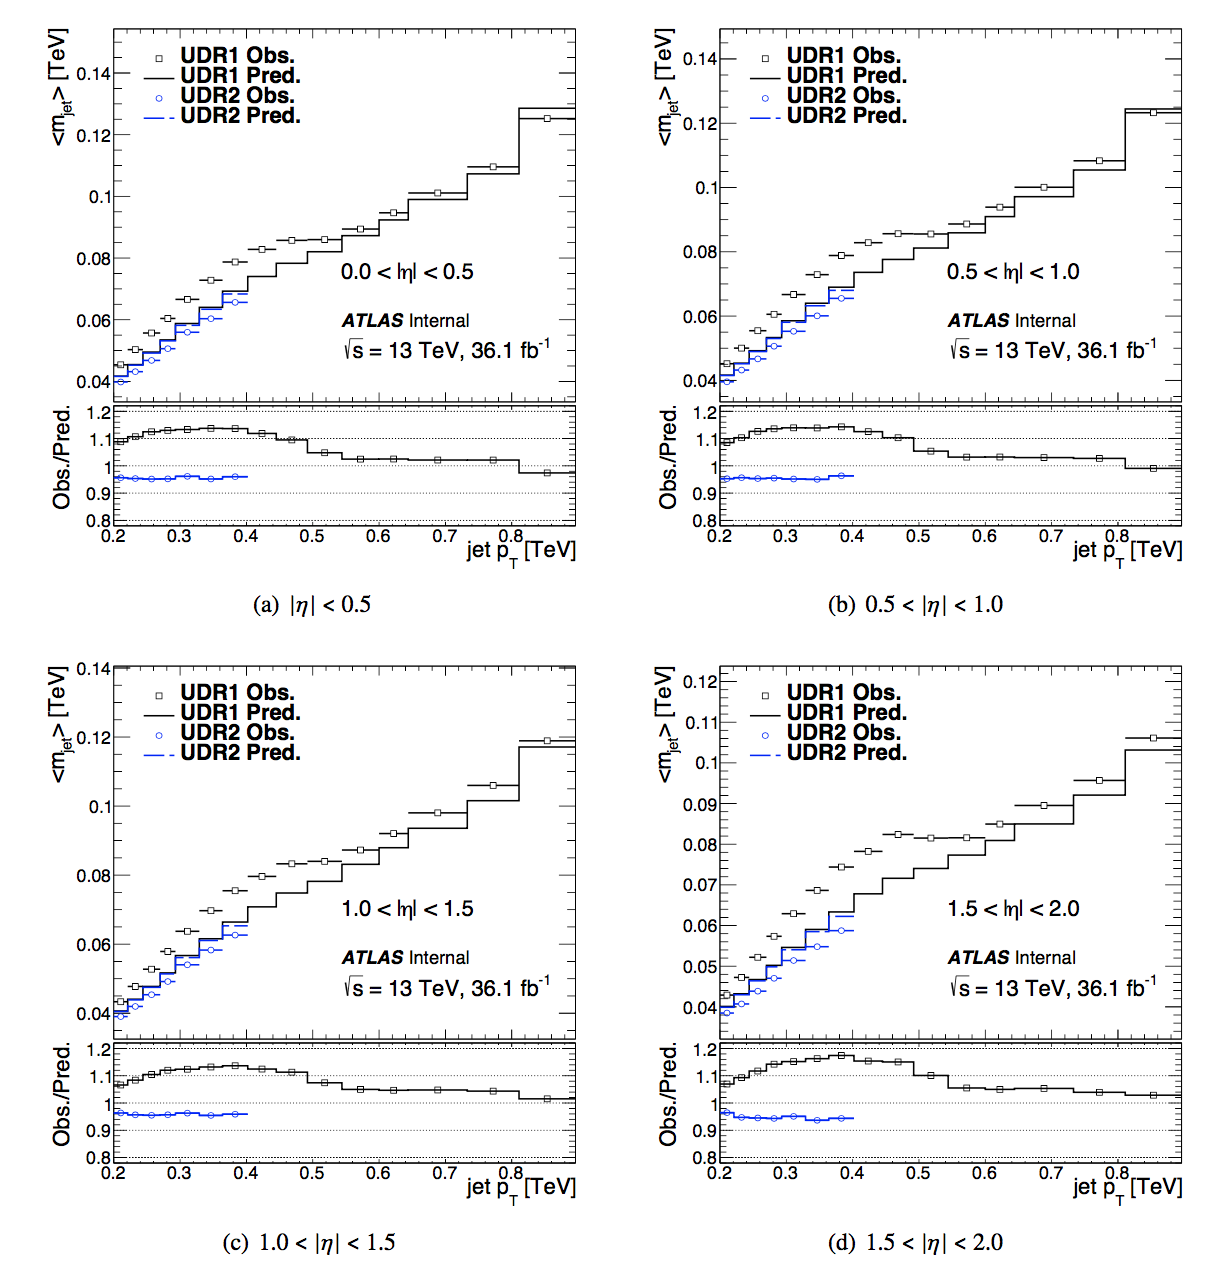
\includegraphics[width=0.9\textwidth]{UDR_response}
    \caption{Jet mass response plots showing the discrepancy between average dressed and kinematic jet masses in the two uncertainty
    determination regions, binned by $p_T$ and $|\eta|$.
    Since the discrepancy is always larger in UDR1, only UDR1 is used to derive uncertainties~\cite{paper-plb}.}
    \label{fig:udr_response}
\end{figure}

Systematic uncertainties are binned in $p_{T}$ and $|\eta|$.
The lowest $p_{T}$ bin is for jets with $p_{T} < 400~GeV$.
The second bin is for jets with $400~GeV \leq p_T < 544~GeV$, and the highest bin is for jets with $p_T \geq 544~GeV$.
For jets with $p_{T} > 400~GeV$, uncertainties are derived only from UDR1.
For jets with $p_{T} < 400~GeV$, uncertainties are derived from both UDR1 and UDR2, and the maximum uncertainty is used.

For each $p_T$ bin in the UDR dressed mass response, a fractional error is calculated as $e_i=\left(<m_{kin}>-<m_{dressed}>\right)/<m_{dressed}>$.
For the lowest and highest $p_T$ systematic bins, the root-mean-square of fractional errors is taken as the systematic error.
For the intermediate systematic bin, the maximum fractional error is taken.

Two separate, uncorrelated systematic uncertainties are derived.
The first uncertainty accounts for the discrepancy between dressed and kinematic masses for jets with $p_T \geq 400~GeV$.
The second accounts for the discrepancy for jets with $p_T < 400~GeV$.
To propagate the low-$p_T$ systematic, two shifted $M_{J}^{\Sigma}$ values are calculated for each dressed $M_{J}^{\Sigma}$.
The first shifted value is obtained by increasing the dressed mass of every low-$p_T$ jet by its corresponding fractional uncertainty.
This yields $n_{toys}$ histograms of shifted $M_{J}^{\Sigma}$.
The average value of each bin content over all toys is taken to obtain the systematically-shifted $M_{J}^{\Sigma}$ distribution.
The second shifted distribution is obtained by \textit{decreasing} the dressed mass of every low-$p_T$ jet by its corresponding fractional uncertainty, and averaging over all the toys to obtain a downwards-shifted distribution of $M_{J}^{\Sigma}$.
The same procedure is used to propagate the high-$p_T$ systematic, but the high-$p_T$ jets are shifted instead of the low-$p_T$ jets.

\section{Effect of signal contamination on background estimation}\label{sec:signal_contamination}
The presence of signal events in the kinematic sample can affect both the nominal background prediction as well as the systematic uncertainty.
This effect can be quantified using a signal injection test.
The background prediction is first calculated from a data sample only, and then calculated from a data sample injected with simulated signal events.

One example of this effect can be seen in figure~\ref{fig:signal_inject_403587}.
For this example, only the first $14.8~fb^{-1}$ of data are used.
The injected signal simulates the cascade decay mode of gluinos with mass $m_{\tilde{g}}=1.8~TeV$ and neutralinos with mass $m_{\tilde{\chi}}=50~GeV$.
For this particular choice of masses and decay mode, signal contamination increases the background prediction by approximately $10\%$, from 18.3 events to 20.2 events.
The systematic uncertainty is increased from 8.9 events to 13.3 events due to the signal contamination.

\begin{figure}[!ht]
    \centering
    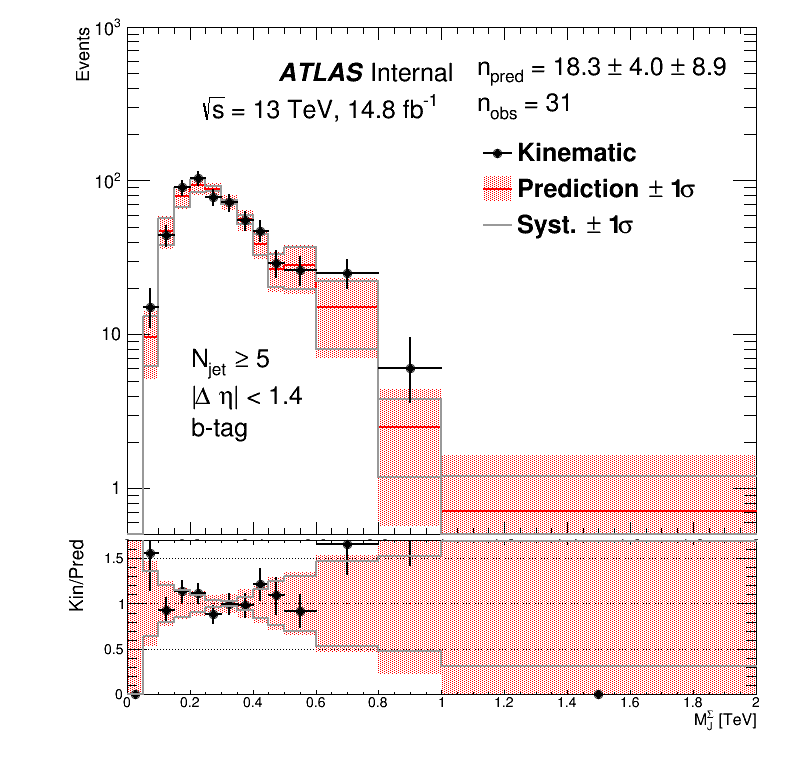
\includegraphics[width=0.45\textwidth]{signal_inject_data_only}
    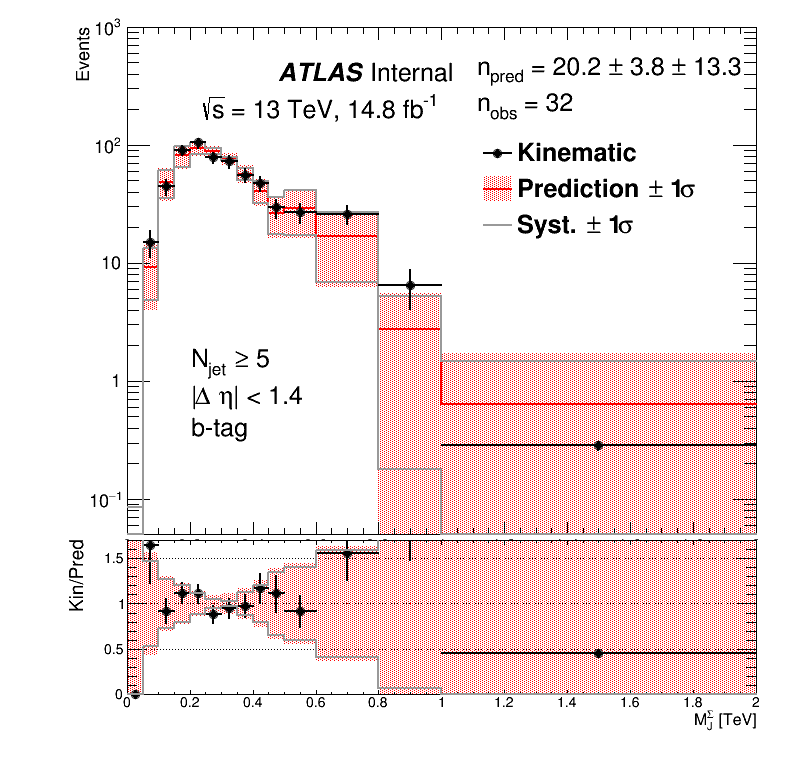
\includegraphics[width=0.45\textwidth]{signal_inject_data_plus_403587}
    \caption{Signal injection test.
    The background prediction is first run only on a data sample (a), and then on a data sample injected with simulated signal events (b).
    The increase in background prediction and systematic uncertainty can be seen.}
    \label{fig:signal_inject_403587}
\end{figure}

The effect of signal contamination on the background prediction has to be measured separately for each pair of $m_{\tilde{g}}$, $m_{\tilde{\chi}}$ values.
For each gluino and neutralino mass point, the background prediction is generated using only simulated signal events in the kinematic sample.
That is, the templates are still derived from data, but the dressing is only performed on simulated signal.
The signal events don't need to be included in the templates because the template control region choice reduces any signal contribution in that region to a negligible amount.
The prediction from the signal-only kinematic sample is then compared to the data-only prediction.
Figure~\ref{fig:signal_contam_grid} shows the ratio of background prediction from signal-only events over the background prediction from data alone.
During hypothesis testing, these ratios will be used to subtract off the signal contamination contribution to the background prediction at each signal point separately.
The signal region used for this test is the 5-jet, b-tag region with $M_J^{\Sigma}>0.8~TeV$ (5jSRb1).

\begin{figure}[!ht]
    \centering
    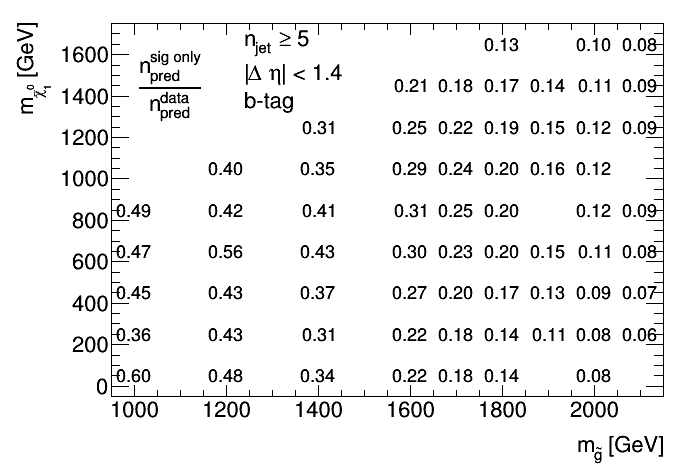
\includegraphics[width=0.75\textwidth]{signal_contam_grid}
    \caption{The effect of signal contamination on the nominal background prediction.
    At each neutralino and gluino mass point, simulated signal events are used in the kinematic sample to generate a background prediction.
    These predictions are compared to the prediction from data only.
    In both cases, the templates are drawn only from data.}
    \label{fig:signal_contam_grid}
\end{figure}

\section{Effect of $t\bar{t}$ on background estimation uncertainty}\label{sec:bkg_ttbar}

Monte Carlo was used to determine if the presence of $t\bar{t}$ events in the uncertainty determination regions would affect the result of the data-driven background estimation.
Figure~\ref{fig:ttbar_UDR1} shows the jet mass response in UDR1 for Pythia8 multijet-only Monte Carlo events and for multi-jet plus $t\bar{t}$.
Figure~\ref{fig:ttbar_UDR1} shows the same comparison for UDR2.
In both cases, the presence of $t\bar{t}$ events has a negligible impact on the resulting uncertainty values.

\begin{figure}[!ht]
    \centering
    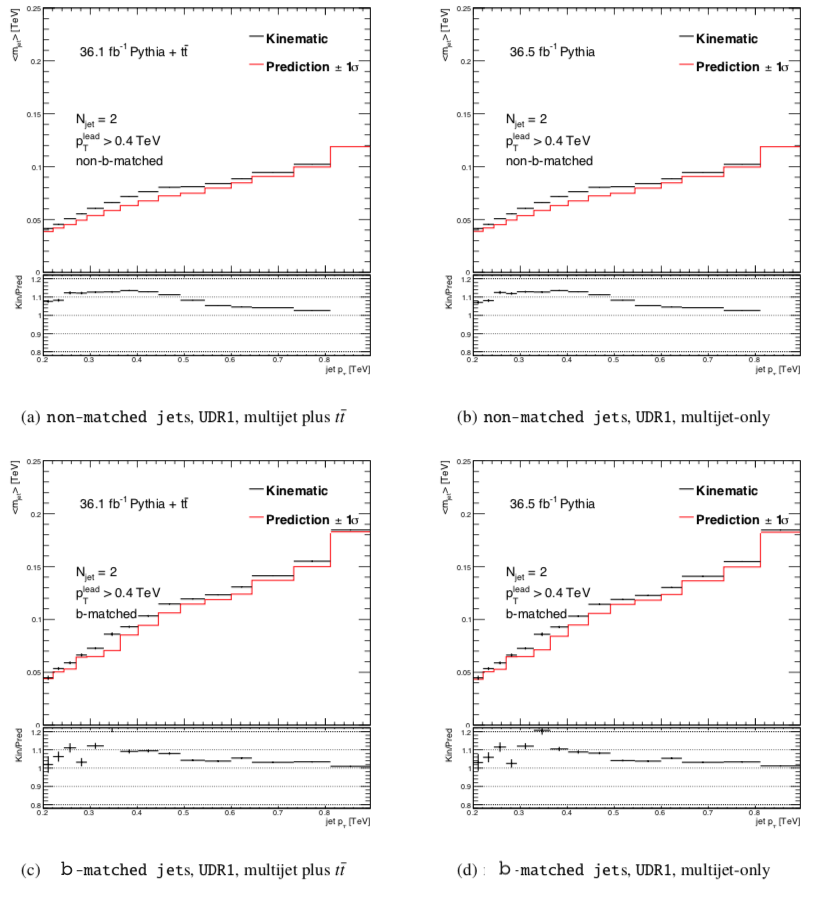
\includegraphics[width=0.9\textwidth]{bkg_ttbar_UDR1}
    \caption{Jet mass response in UDR1 for Pythia8 multijet and $t\bar{t}$ (left column) and Pythia8 multijet only (right column).
    The top two plots show the response for non-b-matched jets only, and the bottom two plots show the response for b-matched jets only.}
    \label{fig:ttbar_UDR1}
\end{figure}

\begin{figure}[!ht]
    \centering
    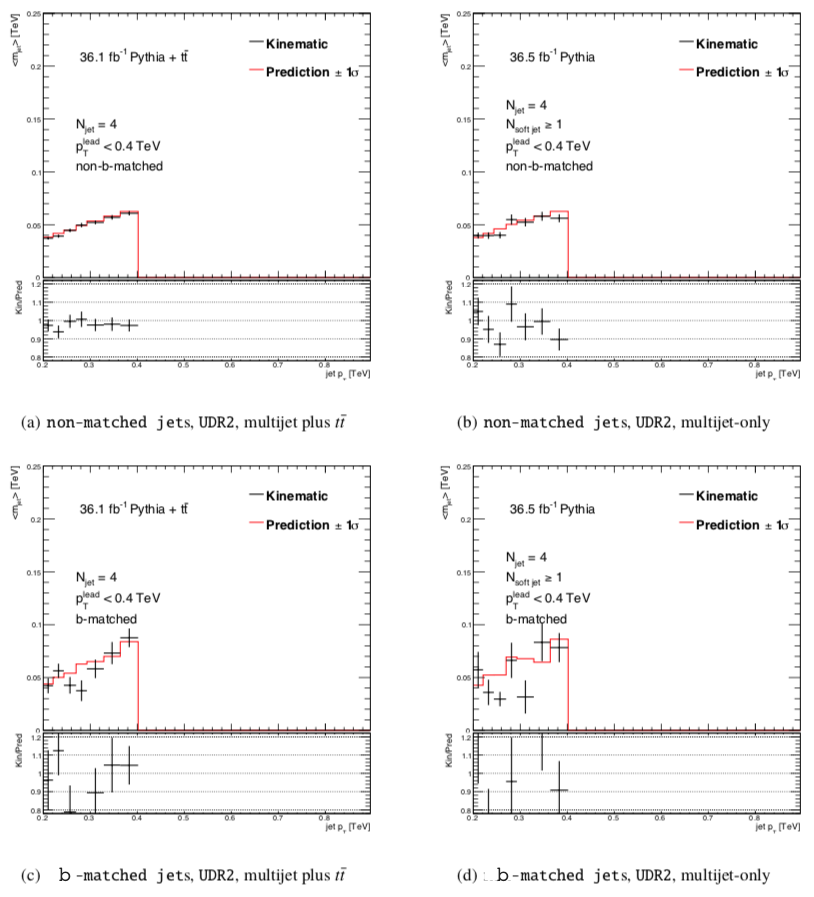
\includegraphics[width=0.9\textwidth]{bkg_ttbar_UDR2}
    \caption{Jet mass response in UDR2 for Pythia8 multijet and $t\bar{t}$ (left column) and Pythia8 multijet only (right column).
    The top two plots show the response for non-b-matched jets only, and the bottom two plots show the response for b-matched jets only.}

    \label{fig:ttbar_UDR2}
\end{figure}

\section{Background estimation method applied to multijet Monte Carlo}\label{sec:bkg_monte_carlo}

The background estimation method was applied to simulated background events from Pythia8 multijets and $t\bar{t}$.
Other multijet Monte Carlo generators were found to disagree significantly with data in the CR and UDRs, and so are not presented here.
The predicted and observed $M_{J}^{\Sigma}$ distributions were compared for the various signal regions, and agreement within uncertainties is observed.
The number of simulated events available resulted in larger statistical uncertainty than is present in data.
The equivalent luminosity available for this study was $1.9~fb^{-1}$.

Figure~\ref{fig:mc_4jSR} shows the predicted and observed $M_{J}^{\Sigma}$ distributions for Pythia8 multijets and $t\bar{t}$ in the $\geq4$-jet b-inclusive region with $|\Delta\eta_{1,2}|<1.4$.
Figure~\ref{fig:mc_4jSRb} shows the same comparison for events with at least one b-tagged jet.
In both cases, there is agreement between the two distributions within systematic uncertainties.
Figures~\ref{fig:mc_5jSR} and~\ref{fig:mc_5jSRb} show similar comparisons for the $\geq5$-jet regions.
In this case the number of simulated events is very small, and so the statistical uncertainty begins to dominate over the systematic uncertainty.
Regardless, the observed $M_{J}^{\Sigma}$ distributions agree with the dressed distributions, within the uncertainties.

This should not be seen as a true test of the background estimation method.
If significant differences between the predicted and observed $M_{J}^{\Sigma}$ distributions \textit{had} been found, it would not necessarily indicate a flaw in the method.
As discussed in~\ref{ch:analysis_overview}, Monte Carlo generators are not expected to perform well in these kinematic regions, hence the need for a data-driven background estimation method in the first place.

\begin{figure}[!ht]
    \centering
    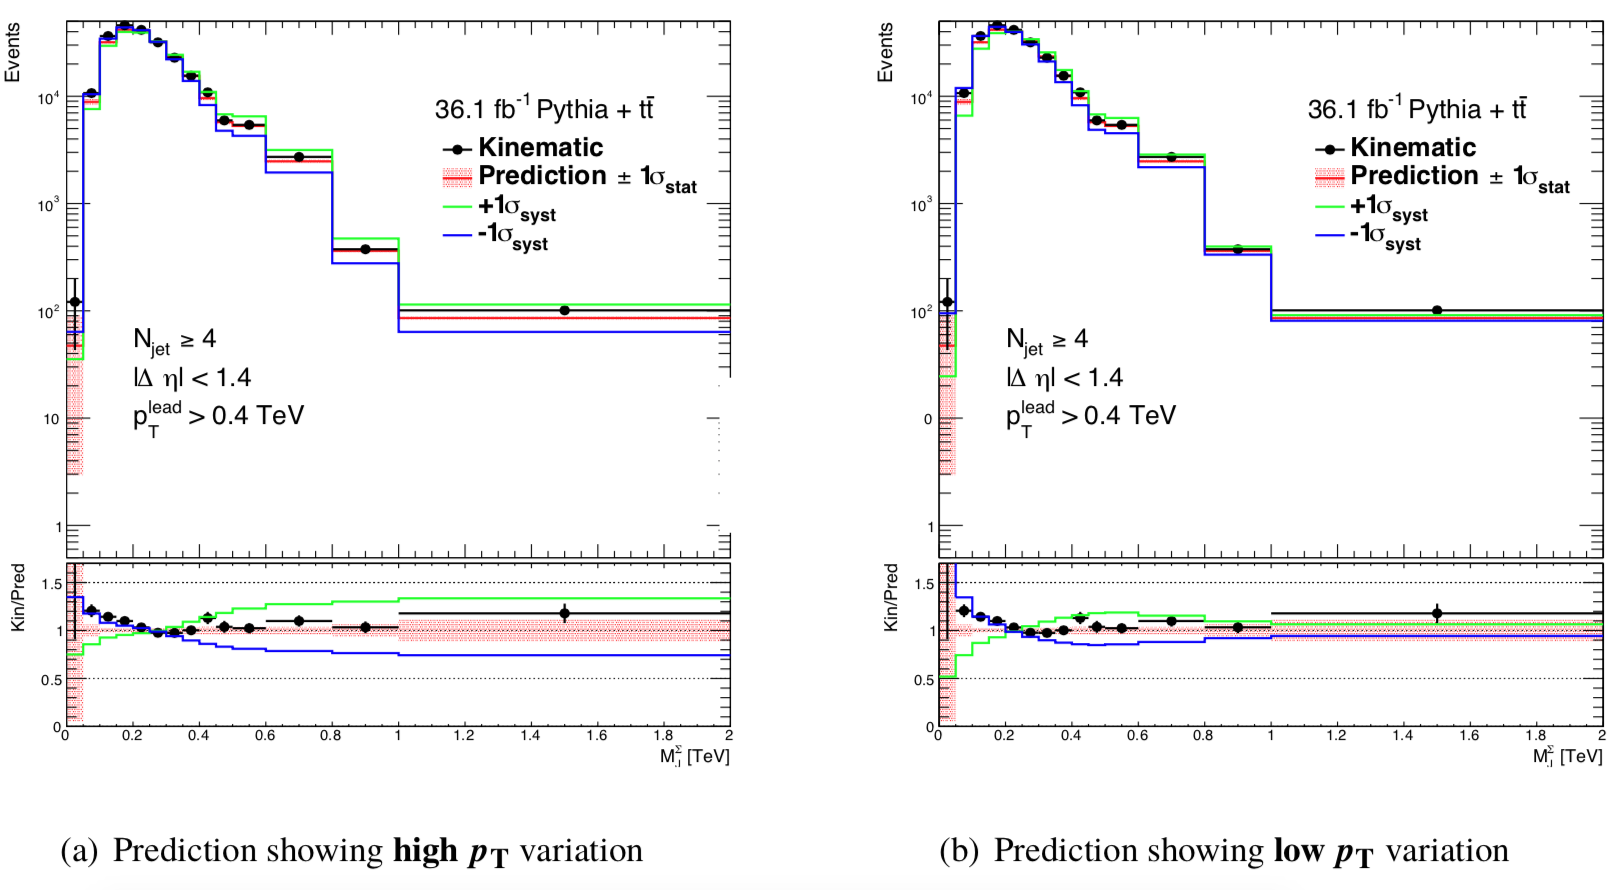
\includegraphics[width=0.9\textwidth]{bkg_mc_4jSR}
    \caption{Predicted and observed $M_{J}^{\Sigma}$ distributions for Pythia8 multijet and $t\bar{t}$ Monte Carlo events in the 4jSR region.
    The red histogram shows the predicted distribution including statistical uncertainty.
    The green and blue histograms show the systematic uncertainty.
    The left plot includes only the high-$p_{T}$ systematic uncertainty, and the right plot shows only the low-$p_{T}$ systematic uncertainty.
    }
    \label{fig:mc_4jSR}
\end{figure}

\begin{figure}[!ht]
    \centering
    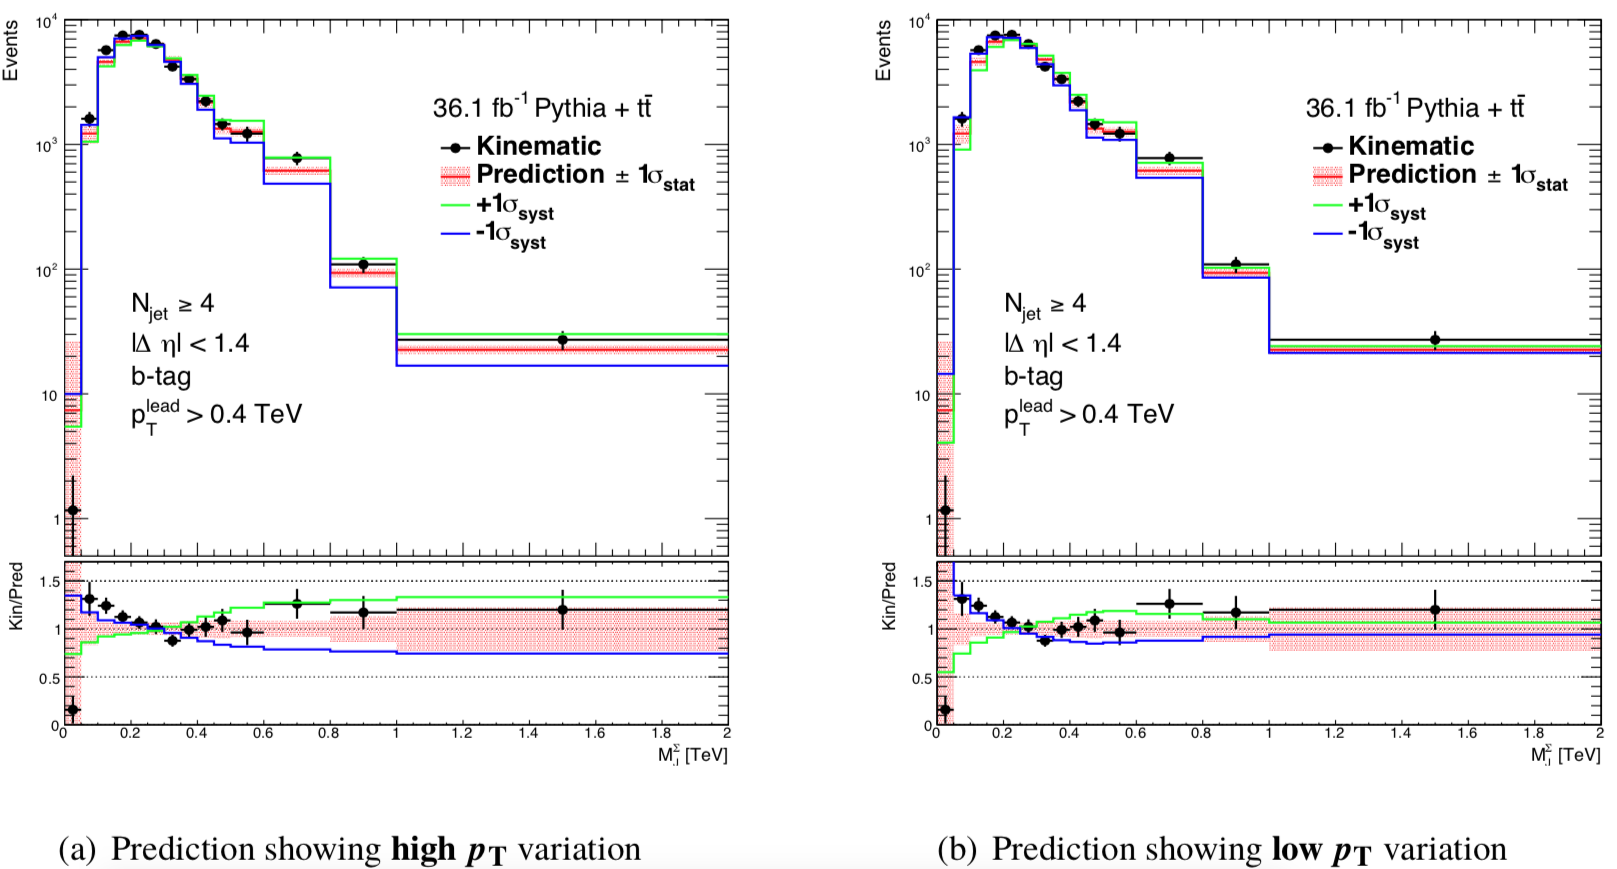
\includegraphics[width=0.9\textwidth]{bkg_mc_4jSRb}
    \caption{Predicted and observed $M_{J}^{\Sigma}$ distributions for Pythia8 multijet and $t\bar{t}$ Monte Carlo events in the 4jSRb region.
    The red histogram shows the predicted distribution including statistical uncertainty.
    The green and blue histograms show the systematic uncertainty.
    The left plot includes only the high-$p_{T}$ systematic uncertainty, and the right plot shows only the low-$p_{T}$ systematic uncertainty.}
    \label{fig:mc_4jSRb}
\end{figure}

\begin{figure}[!ht]
    \centering
    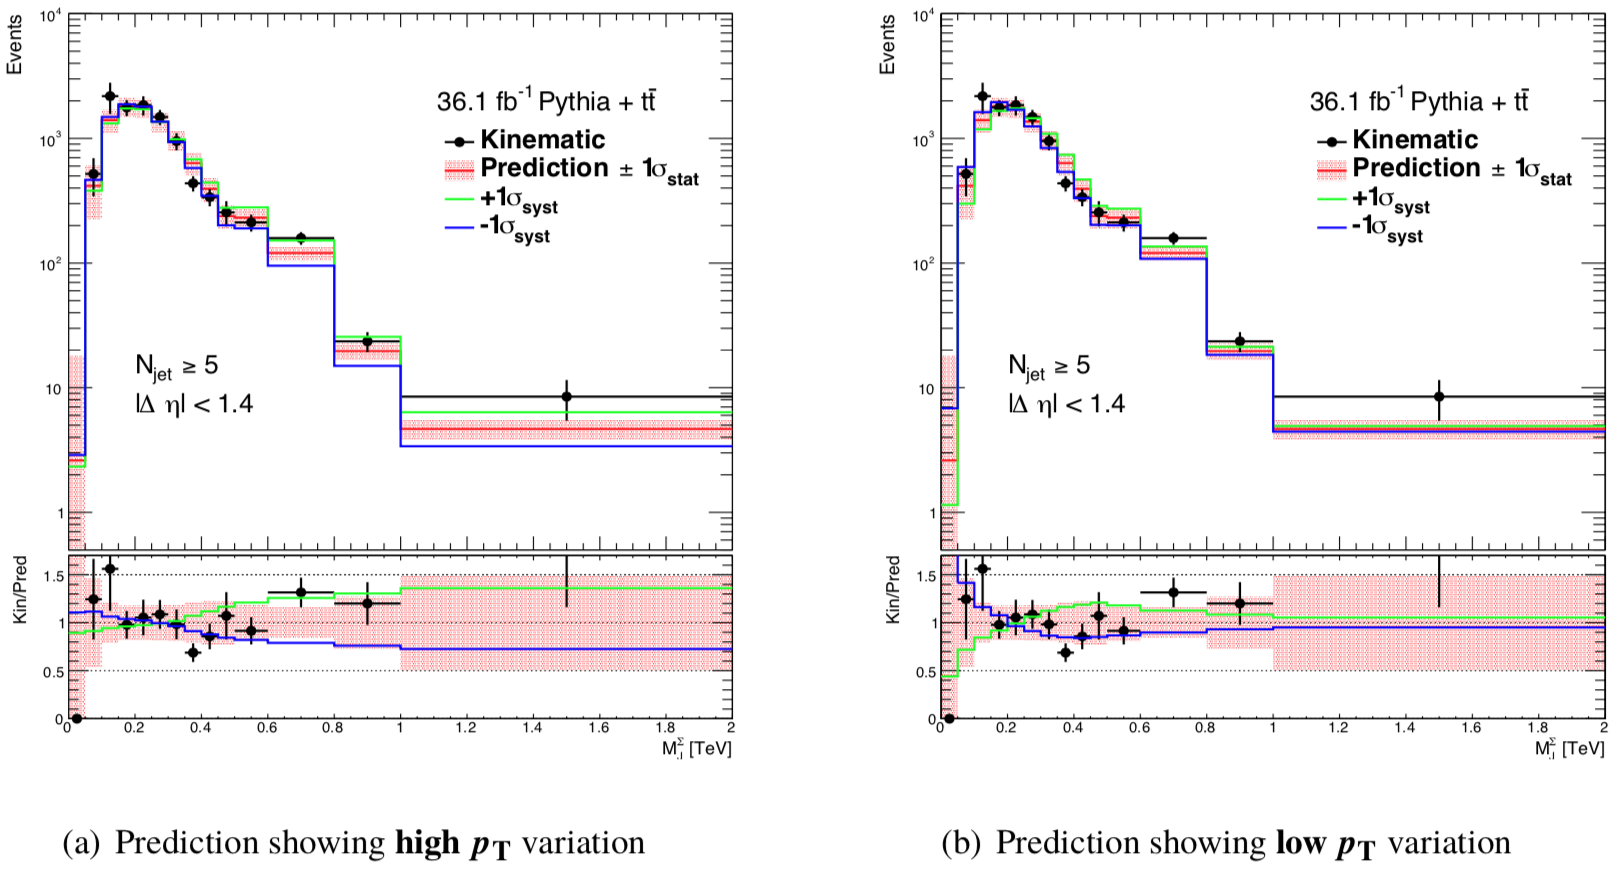
\includegraphics[width=0.9\textwidth]{bkg_mc_5jSR}
    \caption{Predicted and observed $M_{J}^{\Sigma}$ distributions for Pythia8 multijet and $t\bar{t}$ Monte Carlo events in the 5jSR region.
    The red histogram shows the predicted distribution including statistical uncertainty.
    The green and blue histograms show the systematic uncertainty.
    The left plot includes only the high-$p_{T}$ systematic uncertainty, and the right plot shows only the low-$p_{T}$ systematic uncertainty.}
    \label{fig:mc_5jSR}
\end{figure}

\begin{figure}[!ht]
    \centering
    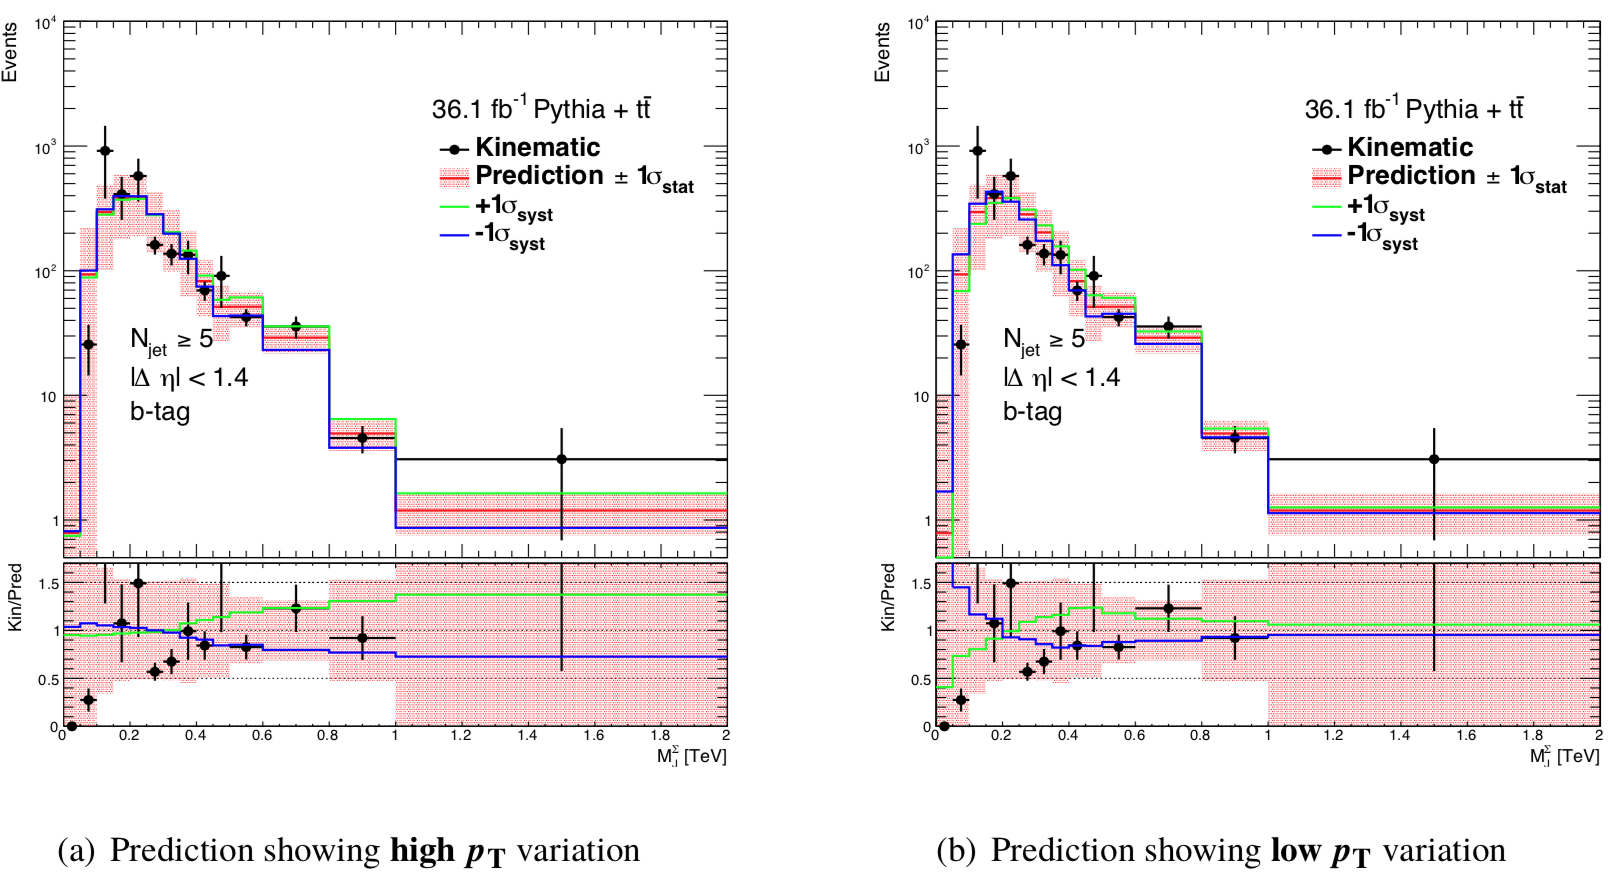
\includegraphics[width=0.9\textwidth]{bkg_mc_5jSRb}
    \caption{Predicted and observed $M_{J}^{\Sigma}$ distributions for Pythia8 multijet and $t\bar{t}$ Monte Carlo events in the 5jSRb region.
    The red histogram shows the predicted distribution including statistical uncertainty.
    The green and blue histograms show the systematic uncertainty.
    The left plot includes only the high-$p_{T}$ systematic uncertainty, and the right plot shows only the low-$p_{T}$ systematic uncertainty.}
    \label{fig:mc_5jSRb}
\end{figure}
